\chapter{Probability Problem set Solutions}
\begin{enumerate}
	\item An unbiased die is cast twice. The probability that the positive difference (bigger smaller) between the two numbers is 2 is
	{\exyear{ JEST 2012}}
	 \begin{tasks}(2)
		\task[\textbf{a.}]$\frac{1}{9}$
		\task[\textbf{b.}]$\frac{2}{9}$
		\task[\textbf{c.}] $\frac{1}{6}$
		\task[\textbf{d.}] $\frac{1}{3}$
	\end{tasks}
	\begin{answer}
		\begin{align*}
		p(2)&=\frac{n(E)}{n(S)}
		\intertext{The number of ways to come positive difference}
		&[(3,1),(4,2),(5,3),(6,4),(1,3)(2,4),(3,5)(4,6)]\\
		p(2)&=\frac{8}{36}=\frac{2}{9}
		\end{align*}
		So the correct answer is \textbf{Option (b)}
	\end{answer}
	\item A box contains 100 coins out of which 99 are fair coins and 1 is a double-headed coin. Suppose you choose a coin at random and toss it 3 times. It turns out that the results of all 3 tosses are heads. What is the probability that the coin you have drawn is the doubleheaded one?
	{\exyear{ JEST 2013}}
	 \begin{tasks}(2)
		\task[\textbf{a.}] $0.99$
		\task[\textbf{b.}]$0.925$
		\task[\textbf{c.}] $0.75$
		\task[\textbf{d.}] $0.01$
	\end{tasks}
	\begin{answer}
		So the correct answer is \textbf{Option (c)}
	\end{answer}
	\item There are on average 20 buses per hour at a point, but at random times. The probability that there are no buses in five minutes is closest to
	{\exyear{ JEST 2013}}
	 \begin{tasks}(2)
		\task[\textbf{a.}]$0.07$
		\task[\textbf{b.}] $0.60$
		\task[\textbf{c.}]$0.36$
		\task[\textbf{d.}] $0.19$
	\end{tasks}
	\begin{answer}
		\begin{align*}
		\intertext{From Poision's distribution function,}
		P(n)&=\frac{e^{-\lambda} \lambda^{n}}{\lfloor n}
		\text{here, }\lambda&=20\text{ buses per hour }\\
		\Rightarrow \lambda&=\frac{5}{3}\text{ buses in five minutes}
		\intertext{Therefore, the probability that there are no buses in five minutes,}
		P(n=0)&=\frac{e^{-\frac{5}{3}}\left(\frac{5}{3}\right)^{0}}{\lfloor 0}=e^{-5 / 3}=0.1886 \approx 0.19
		\end{align*}
		So the correct answer is \textbf{Option (d)}
	\end{answer}
	\item Two drunks start out together at the origin, each having equal probability of making a step simultaneously to the left or right along the $x$ axis. The probability that they meet after $n$ steps is
	{\exyear{ JEST 2013}}
	 \begin{tasks}(2)
		\task[\textbf{a.}]$\frac{1}{4^{n}} \frac{2 n !}{n !^{2}}$
		\task[\textbf{b.}] $\frac{1}{2^{n}} \frac{2 n !}{n !^{2}}$
		\task[\textbf{c.}] $\frac{1}{2^{n}} 2 n !$
		\task[\textbf{d.}]  $\frac{1}{4^{n}} n !$
	\end{tasks}
	\begin{answer}
		\begin{align*}
		\text{The probability of taking ' $r$ '}&\text{ steps out of $N$ steps }={ }^{N} C_{r}\left(\frac{1}{2}\right)^{r}\left(\frac{1}{2}\right)^{N-r}\\
		\text{Total steps }&=N=n+n=2 n
	\intertext{	For taking probability of $n$ steps out of $N$}
	P={ }^{N} C_{n}\left(\frac{1}{2}\right)^{n}\left(\frac{1}{2}\right)^{N-n}&=\frac{N !}{(N-n) ! n !}\left(\frac{1}{2}\right)^{n}\left(\frac{1}{2}\right)^{N-n}=\frac{2 n !}{n ! n !}\left(\frac{1}{2}\right)^{2 n}=\frac{2 n !}{(n !)^{2} 4^{n}}
		\end{align*}
		So the correct answer is \textbf{Option (a)}
	\end{answer}
	\item If two ideal dice are rolled once, what is the probability of getting atleast one '6'?
	{\exyear{ JEST 2015}}
	 \begin{tasks}(2)
		\task[\textbf{a.}]$\frac{11}{36}$
		\task[\textbf{b.}]$\frac{1}{36}$
		\task[\textbf{c.}]$\frac{10}{36}$
		\task[\textbf{d.}]  $\frac{5}{36}$
	\end{tasks}
	\begin{answer}
		\begin{align*}
		\text{Number of point}&\text{ in sample space } n(S)=11\\
		[(1,6),(2,6),(3,6),&(4,6),(5,6),(6,1),(6,2),(6,3),(6,4),(6,5),(6,6)]\\
	\text{	Number of point }&\text{in population }n(P)=6^{2}=36
		\intertext{Probability of getting atleast one '6' on face of dice} &=\frac{n(S)}{n(P)}=\frac{11}{36}
		\end{align*}
			So the correct answer is \textbf{Option (a)}
	\end{answer}
	\item The mean value of random variable $x$ with probability density $p(x)=\frac{1}{\sigma \sqrt{2 \pi}} . \exp \left[-\frac{\left(x^{2}+\mu x\right)}{\left(2 \sigma^{2}\right)}\right]$ is:
	{\exyear{ JEST 2016}}
	 \begin{tasks}(2)
		\task[\textbf{a.}]0
		\task[\textbf{b.}]$\frac{\mu}{2}$
		\task[\textbf{c.}] $\frac{-\mu}{2}$
		\task[\textbf{d.}]  $\sigma$
	\end{tasks}
	\begin{answer}
		\begin{align*}
		\langle x\rangle=\frac{1}{\sigma \sqrt{2 \pi}} \int_{-\infty}^{\infty} x \exp \left(-\frac{x^{2}}{2 \sigma^{2}}\right) d x \int_{-\infty}^{\infty} \exp \left(-\frac{\mu x}{2 \sigma^{2}}\right) d x=0 \quad\text{ (due to odd function)}
		\end{align*}
		So the correct answer is \textbf{Option (a)}
	\end{answer}
\item Suppose that we toss two fair coins hundred times each. The probability that the same number of heads occur for both coins at the end of the experiment is
{\exyear{ JEST 2017}}
 \begin{tasks}(2)
	\task[\textbf{a.}]$\left(\frac{1}{4}\right)^{100} \sum_{n=0}^{100}\left(\begin{array}{c}100 \\ n\end{array}\right)$
	\task[\textbf{b.}] $2\left(\frac{1}{4}\right)^{100} \sum_{n=0}^{100}\left(\begin{array}{c}100 \\ n\end{array}\right)^{2}$
	\task[\textbf{c.}]$\frac{1}{2}\left(\frac{1}{4}\right)^{100} \sum_{n=0}^{100}\left(\begin{array}{c}100 \\ n\end{array}\right)^{2}$
	\task[\textbf{d.}] $\left(\frac{1}{4}\right)^{100} \sum_{n=0}^{100}\left(\begin{array}{c}100 \\ n\end{array}\right)^{2}$
\end{tasks}
\begin{answer}
	\begin{align*}
	\intertext{ If we toss one fair coins hundred times, then probability of $n$ number of head occurs at the end of 100 times is}
	&{ }^{100} C_{n}\left(\frac{1}{2}\right)^{n}\left(\frac{1}{2}\right)^{100-n}
\intertext{	Hence, the probability that same number of heads occur for both coins at the end of experiment is}
&\sum_{n=0}^{100}\left({ }^{100} C_{n}\left(\frac{1}{2}\right)^{100}\right) \cdot\left({ }^{100} C_{n}\left(\frac{1}{2}\right)^{100}\right)=\sum_{n=1}^{100}\left({ }^{100} C_{n}\right)^{2}\left(\frac{1}{2}\right)^{200}=\left(\frac{1}{4}\right)^{100} \sum_{n=1}^{100}\left({ }^{100} C_{n}\right)^{2}
	\end{align*}
		So the correct answer is \textbf{Option (d)}
\end{answer}
\item An electronic circuit with 10000 components performs its intended function success fully with a probability $0.99$ if there are no faulty components in the circuit. The probability that there are faulty components is $0.05$. if there are faulty components, the circuit perform successfully with a probability $0.3$. The probability that the circuit performs successfully is $\frac{x}{10000}$. What is $x$ ?
{\exyear{ JEST 2018}}
\begin{answer}
So the correct answer is  \textbf{9555}
\end{answer}
\item A person plans to go from town $A$ to town $B$ by taking either the route $(R 1+R 2)$ with probability $\frac{1}{2}$ or the route $(R 1+R 3)$ with probability $\frac{1}{2}$ (see figure). Further, there is a probability $\frac{1}{3}$ that $R 1$ is blocked, a probability $\frac{1}{3}$ that $R 2$ is blocked, and a probability $\frac{1}{3}$ that $R 3$ is blocked. What is the probability that he/she would reach town $B$ ?
{\exyear{ JEST 2019}}
\begin{figure}[H]
	\centering
	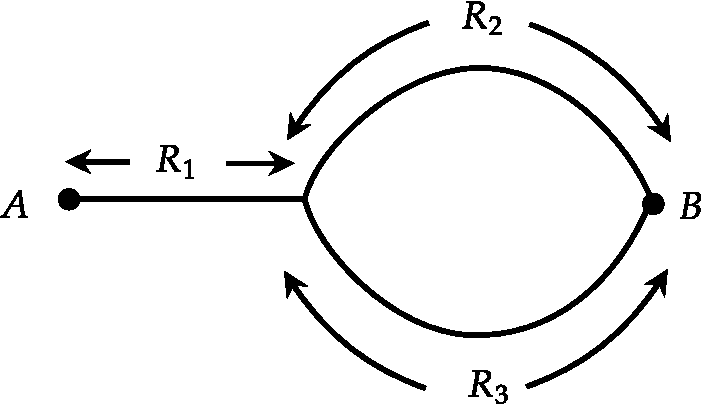
\includegraphics[height=3cm,width=5.5cm]{JEST-58-2019}
\end{figure}
 \begin{tasks}(2)
	\task[\textbf{a.}]$\frac{8}{9}$
	\task[\textbf{b.}]$\frac{1}{3}$
	\task[\textbf{c.}]$\frac{4}{9}$
	\task[\textbf{d.}]$\frac{2}{3}$
\end{tasks}
\begin{answer}
	\begin{align*}
	\text{Given that probability of}&\text{ $R 1$ blocked }=1 / 3\\
	\text{Probability of $R 1$ }&\text{not blocked }=1-\frac{1}{3}=\frac{2}{3}\\
	\text{Probability from $A$ to $B$ }&\text{without restriction }=\frac{1}{2}\\
	\text{Route $R 2$ probability }&=\frac{1}{2} \times \frac{2}{3}\text{ not blocked}\\
	\text{Route }R 3&=\frac{1}{2} \times \frac{2}{3}\\
\text{	Total probability }(A \rightarrow B)&=\frac{2}{3}\left[\frac{1}{2} \times \frac{2}{3}+\frac{1}{2} \times \frac{2}{3}\right]=\frac{4}{9}
	\end{align*}
	So the correct answer is \textbf{Option (c)}
\end{answer}

\end{enumerate}